% 
 	\begin{figure} 
 		\centering
 		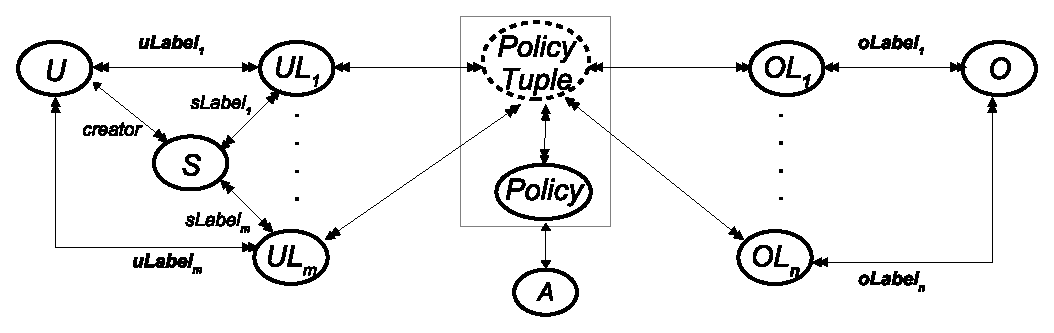
\includegraphics[width=.9\textwidth]{DBSEC16/epabac-mn}
 		\caption{Components of \EPModels{} model with m user and n object attributes}
 		\label{fig:epabac-mn}
 	\end{figure}
 
\label{sec:epmodel}

% 
 	\begin{figure} 
 		\centering
 		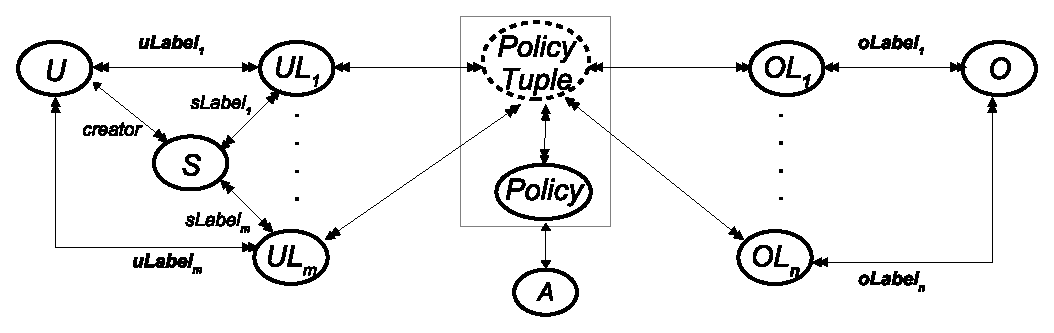
\includegraphics[width=.9\textwidth]{DBSEC16/epabac-mn}
 		\caption{Components of \EPModels{} model with m user and n object attributes}
 		\label{fig:epabac-mn}
 	\end{figure}
 




\begin{table}
	\centering
	\caption{ \EPMNModel{} model} 
	\label{tab:ep-mn-definition}
	%	\begin{tabular}{|l|l|}						
	\begin{tabular}{|l|}

		\hline					
				\begin{tabular}{l}
							\multicolumn{1}{c}{\underline{\textit{I. Sets and relations }}}\\			
							 - $U, O, S, A$ (users, objects, sessions and actions resp)\\
							 - $UL_1, UL_2, ... UL_m$ (values for $\userLabel{1}$, $\userLabel{2}$, ... , $\userLabel{m}$)\\
 							 - $OL_1, OL_2, ... OL_n$ (values for $\objectLabel{1}$, $\objectLabel{2}$, ... , $\objectLabel{n}$)\\
 							 - $uLabel_i: U \to 2 ^ { {UL_i} } $, for $ 1 \le i \le m$; \\
 							 - $oLabel_i: O \to 2 ^ { {OL_i} } $, for $ 1 \le i \le n$\\
 							 - $\creator: S \to U$, many-to-one mapping\\
 							 - $\sessionLabelsP{i}: S \to 2^{\UL{i}} $, for $ 1 \le i \le m$ and $\sessionLabelsP{i}(s) \subseteq \uLabelP{i}(\creator(s))$\\
 							 %- $uLabel_i: U \to 2 ^ {\userLabel{i} }$\\
							 \multicolumn{1}{c}{\underline{\textit{II. Policy components}}} \\	
							 - $\Policy_a \subseteq (2^{\UL{1}} \times 2^{\UL{2}} \times  ... \times 2^{\UL{m}}) \times (2^{\OL{1}} \times 2^{\OL{2}} \times ... \times 2^{\OL{n}})$\\
							 - $\Policy = \{\Policy_a | a \in A \}$\\
								
							\multicolumn{1}{c}{\underline{\textit{III. Authorization function}}} \\						
							 - $\isAuthorized(s:S, a:A, o:O) = (\exists (\ULS{1},\ULS{2}, ..., \ULS{m}, \OLS{1}, \OLS{2}, ... \OLS{n} ) $ \\ \hfill 
							 $ \in \Policy_a)[\ULS{i} = \sessionLabelsP{i}(s), \text{for } 1 \le i \le m \land \OLS{i} = \oLabelP{i}(o), \text{for } 1 \le i \le n]$ 
							 
				\end{tabular}
					
			
 \\ \hline	
	\end{tabular}
	
\end{table}




\EPMNModel{} has \textit{m} user attributes and \textit{n} object attributes. Components of \EPMNModel{}  are shown in Figure \ref{fig:epabac-mn}.  In the figure, the unbounded set of users and objects are shown by the ovals represented by $U$ and $O$. The finite set of actions is represented by the oval $A$. The set of values represented by $\UL{1}, \UL{2}$ through $\UL{m}$ (only $\UL{1} \text{ and } \UL{m}$ are shown in the figure) represent range of $m$ user attribute functions respectively.  $m$ user attributes named $\uLabelP{1}, \uLabelP{2}$ through $\uLabelP{m}$ (only $\uLabelP{1} \text{ and } \uLabelP{m}$ are shown in the figure) are represented by many-to-many connections between users and  corresponding set of values. All these attributes are set valued. Similarly, $\oLabelP{1}, \oLabelP{2} \text{ through } \oLabelP{n}$ denote $n$ object attributes where $\OL{1}$ $\OL{2}$ \text{ through } $\OL{n}$ specify ranges respectively. In an instantiation of the model, it is useful to replace these  attribute names with meaning ones.




The set of policies in this model is shown by the oval $\Policy$. We define at most one policy for a single action. A policy is defined a set of policy tuples. A policy tuple  ($\uVal{1},\uVal{2}, ..., \uVal{m}, \oVal{1},\oVal{2}, ..., \oVal{n}$) takes a subset (including empty set) of values for each user and object attribute.




The set of sessions is represented by the oval S. There is a one-to-many relation between users and sessions. A user can create many sessions but each session must be attached to only one user. The relation $\creator$ between $U$ and $S$ maintains the creating user of a session. In a session, for each user attribute $\uLabelP{i}$, we maintain a relation $\sessionLabelsP{i}$ that maps values of $\uLabelP{i}$ activated by the user. 



The formal definition of the model and semantics of authorization  decision is given in Table \ref{tab:ep-mn-definition}. Segment I of the table defines basic sets and relations discussed above. In Segment II, we show notation of policy tuples and define a policy as a subset of tuples. Finally, the authorization function $\isAuthorized(s,a,o)$ is defined in Segment III.  It allows a session $s$, to perform an action $a$ on an object $o$ if in $\Policy_a$ (the policy for action $a$)  there exists a tuple that satisfies following conditions - (i) values of each user attribute used in the tuple are activated in the session and (ii) values of each object attribute mentioned in the tuple are assigned to  the object.


 
\begin{table*}[t!]
\centering
\caption{User-level session functions in \EPMNModel{}}
\label{tab:ep-abacmn-session}
\begin{tabular}{|l|l|l|}
	\hline
\textbf{Fuction}    & \textbf{Condition} & \textbf{Updates} \\ \hline


\begin{tabular}[c]{@{}l@{}}$\createSession$ $(u:U, s:S, $ \\ $\val{1}:2^{\UL{1}},$ $\val{2}:2^{\UL{2}} $,..., \\ $\val{m}:2^{\UL{m}})$\end{tabular} & \begin{tabular}[c]{@{}l@{}} $u \in U \land s \not \in S \land$  \\$\val{i} \subseteq \ua{i}(u)$, for $1 \le i \le m$\\   \end{tabular} &  \begin{tabular}[c]{@{}l@{}}$S' = S \cup \{s\}$, $\subCreator(s) = u $ , \\ $ \sessionLabelsP{i}(s)=\val{i}$, for $ 1\le i \le m$   \end{tabular} \\\hline


\begin{tabular}[c]{@{}l@{}}$\deleteSession$\\ $(u:U, s:S)$\end{tabular}   & \begin{tabular}[c]{@{}l@{}} $u \in U \land s  \in S \land \subCreator(s)=u  $ \end{tabular}                   & \begin{tabular}[c]{@{}l@{}}$S' = S \setminus \{s\}$ \end{tabular}                             \\\hline

\begin{tabular}[c]{@{}l@{}}$\assignValues$ $(u:U, s:S, $ \\ $\val{1}:2^{\UL{1}},$ $\val{2}:2^{\UL{2}} $,..., \\ $\val{m}:2^{\UL{m}})$\end{tabular} & \begin{tabular}[c]{@{}l@{}} $u \in U \land s  \in S \land \subCreator(s)=u \land $  \\$\val{i} \subseteq \ua{i}(u)$,for $1 \le i \le m$   \end{tabular} &  \begin{tabular}[c]{@{}l@{}} $ \sessionLabelsP{i}'(s)= \sessionLabelsP{i}(s) \cup \val{i}$, \\ for $ 1\le i \le m$   \end{tabular} \\\hline

 \begin{tabular}[c]{@{}l@{}}$\removeValues$ $(u:U, s:S, $ \\ $\val{1}:2^{\UL{1}},$ $\val{2}:2^{\UL{2}} $,..., \\ $\val{m}:2^{\UL{m}})$\end{tabular} & \begin{tabular}[c]{@{}l@{}} $u \in U \land s  \in S \land \subCreator(s)=u \land $  \\   \end{tabular} &  \begin{tabular}[c]{@{}l@{}} $  \sessionLabelsP{i}'(s)= \sessionLabelsP{i}(s) \setminus \val{i}$   \end{tabular} \\\hline
                 
\end{tabular}
\end{table*}
 
%
 	\begin{figure} 
 		\centering
 		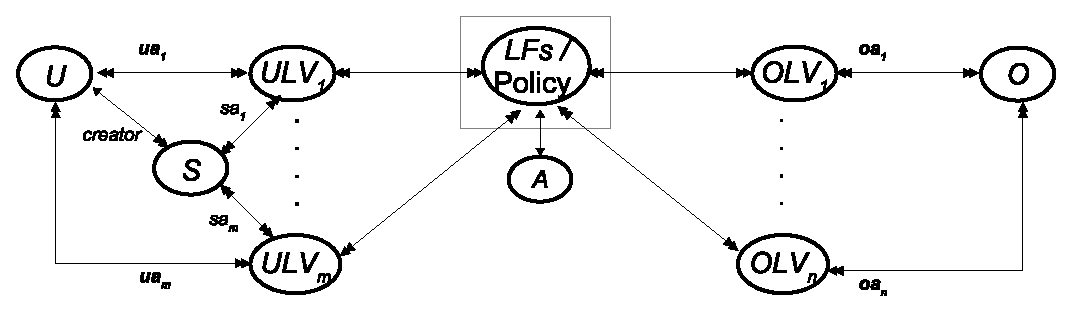
\includegraphics[width=.9\textwidth]{DBSEC16/lpabac-mn}
 		\caption{Components of \LPModels{} model with m user and n object attributes}
 		\label{fig:lp-abacmn-diagram}
 	\end{figure}

User-level session management functions of \EPMNModel{} are given in Table \ref{tab:ep-abacmn-session}. \EPMNModel{} allows users to create or destroy sessions, assign or remove values to attributes in a session.  In Table \ref{tab:ep-abacmn-session}, each session function is specified with its formal parameters, necessary preconditions and resulting updates as shown in $1^{st}, 2^{nd} \text{ and }  3^{rd}$ columns respectively. The function $\createSession()$ creates a new session with given values and $\deleteSession()$ deletes an existing session.  $\assignValues()$ and $\removeValues()$  assign or remove attributes values of an existing session.




